\documentclass[a4paper,14pt]{extarticle}
\usepackage[top=1in,bottom=1in,left=1in,right=1in]{geometry}
\setlength{\emergencystretch}{2em}  % Allows some flexibility in line breaking
\usepackage{amsmath}
\usepackage{amssymb}
\usepackage{graphicx}
\usepackage{fontspec}
\usepackage{hyperref}

% Required packages
\usepackage{thmtools}
\usepackage{tikz}
\usepackage{xcolor}
\usepackage{mdframed}

% Define colors
\definecolor{contextcolor}{RGB}{240,248,255}  % Light blue
\definecolor{setupcolor}{RGB}{245,245,245}    % Light gray
\definecolor{thinkcolor}{RGB}{230,245,230}    % Light green

% Define counter for exercises
\newcounter{exercisecount}

% Define custom commands
\newcommand{\exercise}[1][]{%
    \stepcounter{exercisecount}%
    \phantomsection % Add anchor for hyperref
    \addcontentsline{toc}{section}{Exercise \theexercisecount: #1} % Add to table of contents
    \section*{\large\textbf{Exercise \theexercisecount:} #1}\par\medskip}

% Define custom commands
\newcounter{stepcount}[exercisecount]
\newcommand{\step}{\stepcounter{stepcount}\paragraph{Step \theexercisecount.\thestepcount}}
\newcommand{\think}[1]{
    \begin{mdframed}[backgroundcolor=thinkcolor,linewidth=0.5pt]
    \textit{Think:} #1
    \end{mdframed}}

% Document settings
\setlength{\parindent}{0pt}
\setlength{\parskip}{1em}

\usetikzlibrary{calc,decorations,patterns,arrows,decorations.pathmorphing,positioning}
\definecolor{pltblue}{HTML}{1F77B4}
\tikzset{every picture/.style={/utils/exec={\fontspec{Pretty Neat}}}}
\setmainfont{Pretty Neat}

\usepackage{wasysym}  % Provides \Square symbol

\makeatletter
\pgfset{
  /pgf/decoration/randomness/.initial=2,
  /pgf/decoration/wavelength/.initial=100
}
\pgfdeclaredecoration{sketch}{init}{
  \state{init}[width=0pt,next state=draw,persistent precomputation={
    \pgfmathsetmacro\pgf@lib@dec@sketch@t0
  }]{}
  \state{draw}[width=\pgfdecorationsegmentlength,
  auto corner on length=\pgfdecorationsegmentlength,
  persistent precomputation={
    \pgfmathsetmacro\pgf@lib@dec@sketch@t{mod(\pgf@lib@dec@sketch@t+pow(\pgfkeysvalueof{/pgf/decoration/randomness},rand),\pgfkeysvalueof{/pgf/decoration/wavelength})}
  }]{
    \pgfmathparse{sin(2*\pgf@lib@dec@sketch@t*pi/\pgfkeysvalueof{/pgf/decoration/wavelength} r)}
    \pgfpathlineto{\pgfqpoint{\pgfdecorationsegmentlength}{\pgfmathresult\pgfdecorationsegmentamplitude}}
  }
  \state{final}{}
}
\tikzset{xkcd/.style={decorate,decoration={sketch,segment length=0.5pt,amplitude=0.5pt}}}
\makeatother

\usepackage{etoolbox}
\AtBeginEnvironment{tabular}{\fontspec{Pretty Neat}}

\setlength{\parindent}{0pt}
\setlength{\parskip}{0.5em}
\usepackage{fancyhdr}
\usepackage{adjustbox}
\usepackage{titling}
\usepackage{multicol}
\usepackage{enumitem}

\title{Random Walk Characteristics Worksheet}
\author{Network Science Course}
\date{}

\begin{document}

\exercise[Building RNNs: From Rolling Balls to Hidden States]

\step Imagine a ball rolling on a surface with air resistance (drag). The ball's momentum (hidden state) changes based on:
\begin{enumerate}
    \item Previous momentum (how fast it was already rolling)
    \item New external force (input)
\end{enumerate}

For force sequence [1, 1, 1, 1], shade boxes to show momentum (white = 0 m/s, light gray = 1 m/s, medium gray = 2 m/s, dark gray = 3 m/s, black = 4+ m/s):

\begin{center}
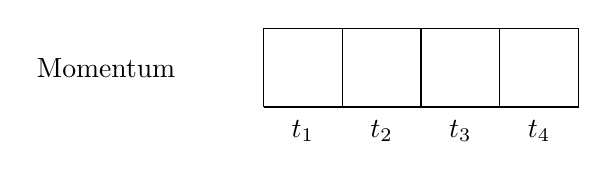
\begin{tikzpicture}
    \begin{scope}[yshift=0cm]
        \draw (0,0) grid[step=1] (4,1);
        \foreach \x/\t in {0.5/$t_1$, 1.5/$t_2$, 2.5/$t_3$, 3.5/$t_4$} {
            \node[rotate=0] at (\x,-0.3) {\t};
        }
        \node at (-2,0.5) {Momentum};
    \end{scope}
\end{tikzpicture}
\end{center}

\step In both physics and RNNs, we need a way to control how much past information is retained. In physics, this is air resistance (drag), which reduces velocity proportionally to speed. In RNNs, we use a weight ($w$) that serves the same purpose - it determines what fraction of the previous momentum is kept. A high weight ($w = 0.9$) means 90\% of momentum is retained (low drag), while a low weight ($w = 0.1$) means only 10\% is retained (high drag).

For force sequence [2, 2, 0, 0], shade three sets of boxes for:
\begin{enumerate}[label=(\alph*)]
    \item High retention ($w = 0.9$)
    \item Medium retention ($w = 0.5$)
    \item Low retention ($w = 0.1$)
\end{enumerate}

\begin{center}
\begin{tikzpicture}
    \begin{scope}[yshift=4cm]
        \draw (0,0) grid[step=1] (4,1);
        \node at (-2,0.5) {$w = 0.9$};
    \end{scope}
    \begin{scope}[yshift=2cm]
        \draw (0,0) grid[step=1] (4,1);
        \node at (-2,0.5) {$w = 0.5$};
    \end{scope}
    \begin{scope}[yshift=0cm]
        \draw (0,0) grid[step=1] (4,1);
        \node at (-2,0.5) {$w = 0.1$};
    \end{scope}
\end{tikzpicture}
\end{center}

\think{How does $w$ affect the network's memory of past inputs?}

\step Just as real objects can't have infinite speed due to air resistance, RNNs need a way to prevent unbounded growth of the hidden state. We introduce the $\tanh$ activation function as our "speed limit." Let's see how our physical model becomes an RNN:

Physical model: $\text{new momentum} = w \times \text{old momentum} + w_x \times \text{force}$
RNN model: $h_{\text{new}} = \tanh(w \times h_{\text{old}} + w_x \times \text{force})$

where:
\begin{enumerate}
    \item $h_{\text{old}}$ is previous momentum
    \item $\text{force}$ is input
    \item $w$ controls memory retention (like inverse drag coefficient)
    \item $w_x$ controls force sensitivity
    \item $\tanh$ keeps values between -1 and 1 (our speed limit)
\end{enumerate}

For these force sequences, shade the predicted momentum (white = -1, light gray = -0.5, medium gray = 0, dark gray = 0.5, black = 1), with $w = 1.0$ and $w_x = 1$:

\begin{center}
\begin{tabular}{ccc}
    [3,0,0,0] & [1,1,1,1] & [0,3,0,0] \\
    \begin{tabular}{|c|c|c|c|}
    \hline
    $\square$ & $\square$ & $\square$ & $\square$ \\
    \hline
    \end{tabular}
    &
    \begin{tabular}{|c|c|c|c|}
    \hline
    $\square$ & $\square$ & $\square$ & $\square$ \\
    \hline
    \end{tabular}
    &
    \begin{tabular}{|c|c|c|c|}
    \hline
    $\square$ & $\square$ & $\square$ & $\square$ \\
    \hline
    \end{tabular}
\end{tabular}
\end{center}

\think{How does each force sequence affect momentum differently? Which sequence would be hardest for the network to "learn"?}

\step Design your own RNN weights! If you wanted to: (Design 1) Remember past inputs longer, (Design 2) Respond more quickly to new forces, (Design 3) Have a maximum speed limit. Shade these weight matrices (white = 0, black = 1) to achieve each goal:

\begin{center}
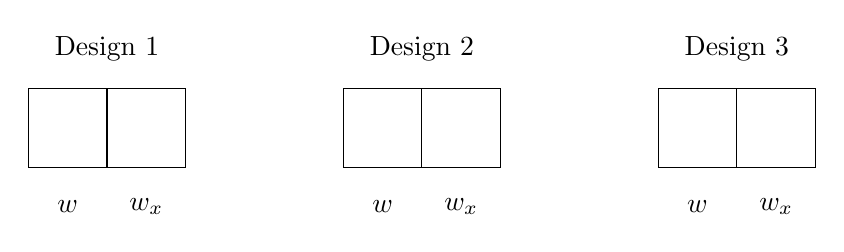
\begin{tikzpicture}
    \begin{scope}[yshift=0cm]
        \draw (0,0) grid[step=1] (2,1);
        \draw (4,0) grid[step=1] (6,1);
        \draw (8,0) grid[step=1] (10,1);
        \node at (1,1.5) {Design 1};
        \node at (5,1.5) {Design 2};
        \node at (9,1.5) {Design 3};
        \node at (0.5,-0.5) {$w$};
        \node at (1.5,-0.5) {$w_x$};
        \node at (4.5,-0.5) {$w$};
        \node at (5.5,-0.5) {$w_x$};
        \node at (8.5,-0.5) {$w$};
        \node at (9.5,-0.5) {$w_x$};
    \end{scope}
\end{tikzpicture}
\end{center}

\step Predict what would happen with these "physically impossible" weights:
\begin{enumerate}
    \item $w > 1$ (momentum grows from previous state)
    \item No activation function
    \item Negative weights
\end{enumerate}

Shade the momentum evolution for input sequence [1, 1, 1, 1] (use white = minimum value, black = maximum value in each case):

\begin{center}
\begin{tikzpicture}
    \begin{scope}[yshift=0cm]
        \draw (0,0) grid[step=1] (4,1);
        \draw (0,2) grid[step=1] (4,3);
        \draw (0,4) grid[step=1] (4,5);
        \node at (-1.5,4.5) {$w = 1.2$};
        \node at (-1.5,2.5) {No tanh};
        \node at (-1.5,0.5) {$w = -0.5$};
    \end{scope}
\end{tikzpicture}
\end{center}

\think{Why are these scenarios "impossible" physically but possible in an RNN? What problems might they cause or solve?}

\end{document}